% !TEX program=lualatex
\RequirePackage{luatex85}
\documentclass[11pt,tikz]{standalone}

\usepackage{luatextra} % also loads fixltx2e, fontspec, xunicode
\usepackage{microtype} % Slightly tweak font spacing for aesthetics
\usepackage{mathtools}
\usepackage{amsmath}
\usepackage{unicode-math}
\usepackage{xcolor}

\usepackage{tikz}
\usetikzlibrary{shapes,arrows,positioning,matrix,fit}

\setmainfont{TeX Gyre Heros}
\setmathfont{Latin Modern Math}
\setmonofont{Source Code Pro}

\definecolor{colorR}{RGB}{228,26,28}    % RED
\definecolor{colorB}{RGB}{55,126,184}   % BLUE
\definecolor{colorG}{RGB}{77,175,74}    % GREEN
\definecolor{colorP}{RGB}{152,78,163}   % PURPLE
\definecolor{colorO}{RGB}{255,127,0}    % ORANGE
\definecolor{colorY}{RGB}{255,255,51}   % YELLOW
\definecolor{colorBn}{RGB}{166,86,40}   % BROWN
\definecolor{colorPk}{RGB}{247,129,191} % PINK
\definecolor{colorGy}{RGB}{153,153,153} % GRAY
\definecolor{asublue}{RGB}{0,163,224}

\tikzstyle{aln}=[matrix of nodes, nodes in empty cells]
%\tikzstyle{best}=[fill=asublue!20,rounded corners]
\tikzstyle{best}=[rounded corners]
\tikzstyle{lab}=[font=\normalsize]
\tikzstyle{indel}=[ultra thick, rounded corners]
\tikzstyle{phase0}=[draw=colorGy]
\tikzstyle{phase1}=[draw=colorP]
\tikzstyle{phase2}=[draw=colorO]

\newcommand{\e}[1]{\textbf{\textcolor{colorR}{#1}}}

\begin{document}
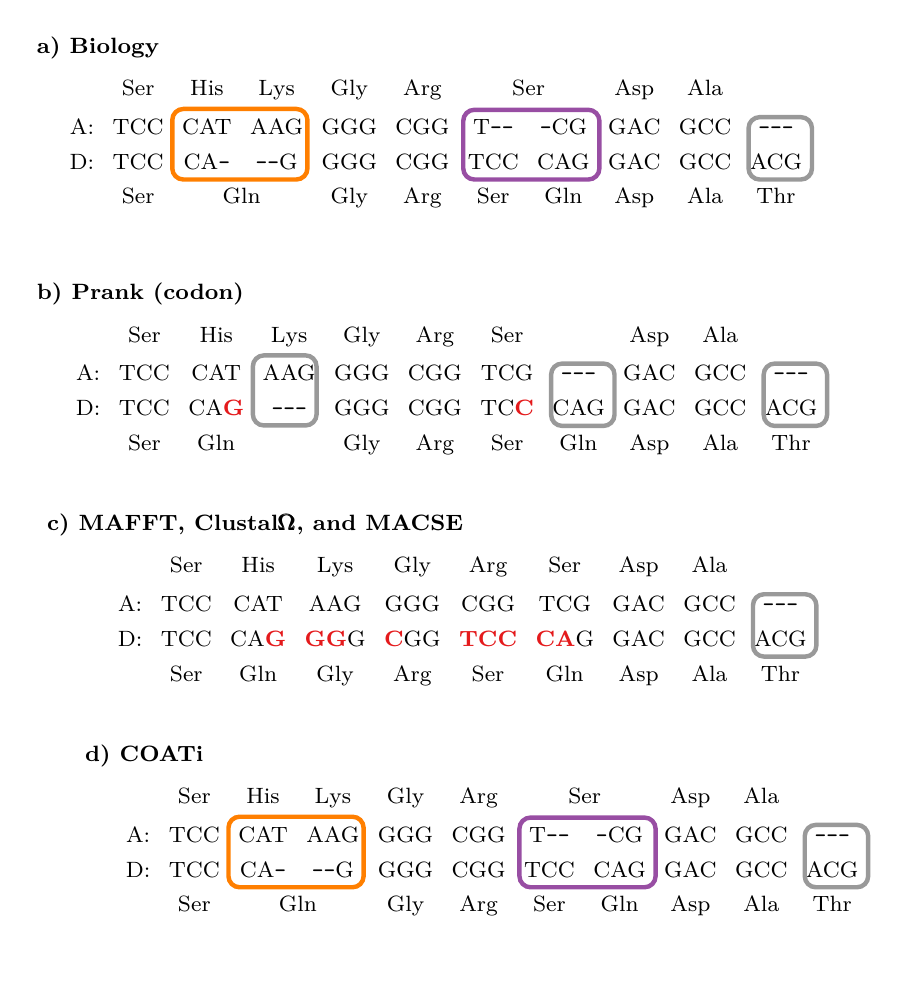
\begin{tikzpicture}[node distance=5mm,font=\footnotesize]

\node (titleBiology) {\textbf{a) Biology}};
% biology
\matrix (biology)[aln,best,below right=-1mm and -15mm of titleBiology] {
   & Ser & His & Lys & Gly & Arg &            &            & Asp & Ala & \\
A: & TCC & CAT & AAG & GGG & CGG & T\verb|--| & \verb|-|CG & GAC & GCC & \verb|---|\\
D: & TCC & CA\verb|-| & \verb|--|G & GGG & CGG & TCC & CAG & GAC & GCC & ACG\\
   & Ser &            &            & Gly & Arg & Ser & Gln & Asp & Ala & Thr\\
};
\node (bio17) [fit=(biology-1-7)(biology-1-8)]{Ser};
\node [fit=(biology-4-3)(biology-4-4)]{Gln};
\draw [indel,phase1] (biology-2-7.north west) rectangle (biology-3-8.south east);
\draw [indel,phase0] (biology-2-11.north west) rectangle (biology-3-11.south east);
\draw [indel,phase2] (biology-2-3.north west) rectangle (biology-3-4.south east);


\node (titlePrank) [below right=2.6cm and -1.8cm of titleBiology] {\textbf{b) Prank (codon)}};
% prank codon --gaprate=0.01
\matrix (prank) [aln,below right=-1mm and -2.5cm of titlePrank] {
   & Ser & His     & Lys & Gly  & Arg & Ser &           & Asp & Ala & \\
A: & TCC & CAT     & AAG & GGG  & CGG & TCG &\verb|---| & GAC & GCC & \verb|---|\\
D: & TCC & CA\e{G} & \verb|---| & GGG & CGG & TC\e{C} & CAG & GAC & GCC & ACG\\
   & Ser & Gln     &            & Gly     & Arg & Ser   & Gln  & Asp & Ala & Thr\\
};
\draw [indel,phase0] (prank-2-8.north west) rectangle (prank-3-8.south east);
\draw [indel,phase0] (prank-2-11.north west) rectangle (prank-3-11.south east);
\draw [indel,phase0] (prank-2-4.north west) rectangle (prank-3-4.south east);

\node (titleMafftClustalo) [below right=2.4cm and -2.75cm of titlePrank] {\textbf{c) MAFFT, Clustal$\pmb{\Omega}$, and MACSE}};
% mafft dna & clustalo amino acids
\matrix(mafft-clustalo) [aln,below right=-1mm and -4.75cm of titleMafftClustalo] {
   & Ser & His     & Lys     & Gly     & Arg     & Ser & Asp & Ala & \\
A: & TCC & CAT & AAG & GGG     & CGG     & TCG & GAC & GCC & \verb|---|\\
D: & TCC & CA\e{G}     & \e{GG}G     & \e{C}GG & \e{TCC} & \e{CA}G & GAC & GCC & ACG\\
   & Ser & Gln     & Gly     & Arg     & Ser     & Gln & Asp & Ala & Thr\\
};
\draw [indel,phase0] (mafft-clustalo-2-10.north west) rectangle (mafft-clustalo-3-10.south east);

\node (titleCoati) [below right=2.4cm and -5.05cm of titleMafftClustalo] {\textbf{d) COATi}};
% coati mar-mg
\matrix (coati) [aln,best,below right=-1mm and -1.35cm of titleCoati] {
   & Ser & His & Lys & Gly & Arg &            &            & Asp & Ala & \\
A: & TCC & CAT & AAG & GGG & CGG & T\verb|--| & \verb|-|CG & GAC & GCC & \verb|---|\\
D: & TCC & CA\verb|-| & \verb|--|G & GGG & CGG & TCC & CAG & GAC & GCC & ACG\\
   & Ser &            &            & Gly & Arg & Ser & Gln & Asp & Ala & Thr\\
};
\node (cti17) [fit=(coati-1-7)(coati-1-8)]{Ser};
\node [fit=(coati-4-3)(coati-4-4)]{Gln};
\draw [indel,phase1] (coati-2-7.north west) rectangle (coati-3-8.south east);
\draw [indel,phase0] (coati-2-11.north west) rectangle (coati-3-11.south east);
\draw [indel,phase2] (coati-2-3.north west) rectangle (coati-3-4.south east);

%%%%%

% \draw (a.north west) node[lab,anchor=center] (dlab) {\textbf{a)}};
% \draw (dlab |- c.north west) node[lab,anchor=center] {\textbf{b)}};

\node[] () [below = 0.2em] at (coati.south) {};

\end{tikzpicture}
\end{document}
